\subsectionfont{\fontsize{14}{14}\selectfont}


\subsection{Dashboard}
The user interface showcases a dashboard that displays real-time rocket telemetry data on the Home page. 
It features a "Satellites in View" widget that displays satellites that are utilized by the rocket, as well as 
various graphs that plot data received from the backend via a WebSocket. All visuals are updated in real-time as
the data is received, providing the user with a realistic view of the rocket's current status. 

\begin{figure}[H]
    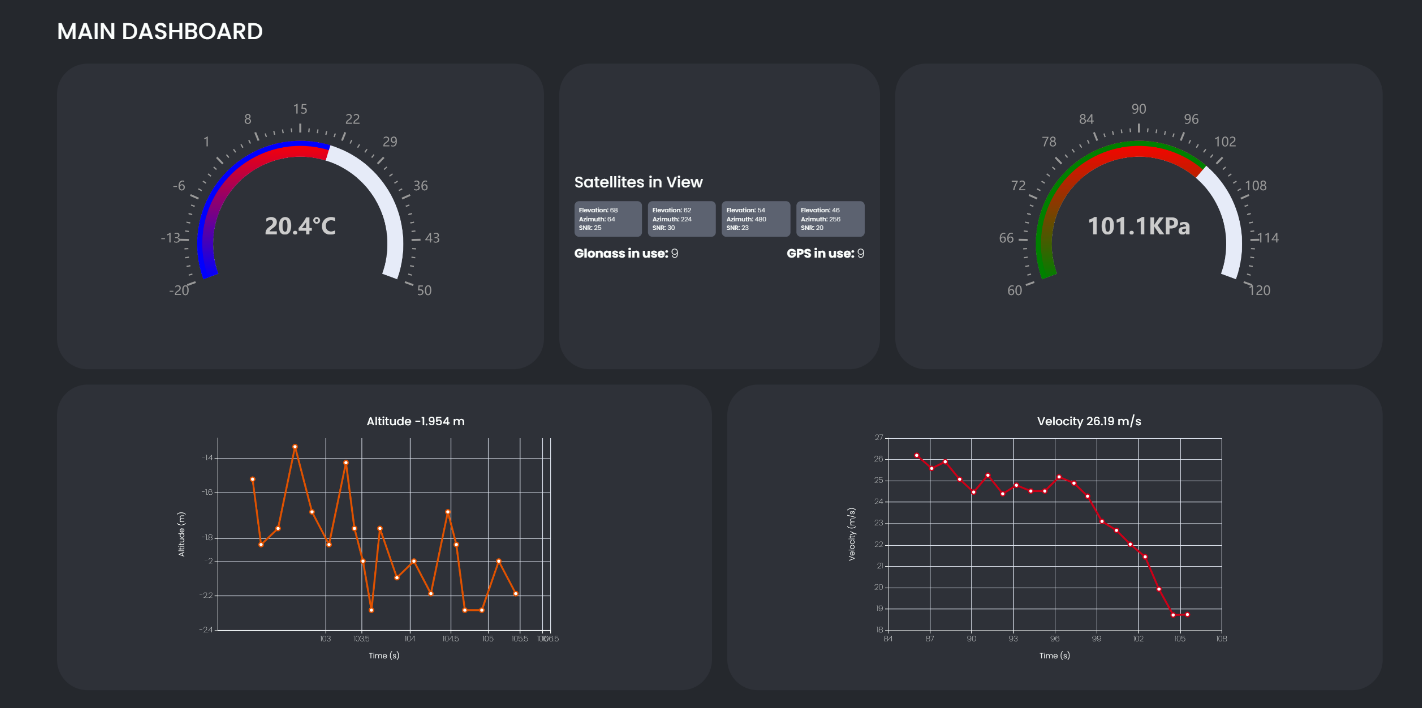
\includegraphics [scale=0.75] {ui_dashboard}
    \centering
    \captionof{figure} {The dashboard of the user interface}
\end{figure}

\subsubsection {Satellites in View}
The "Satellites in View" widget displays the number of GLONASS and GPS satellites that are being used by the 
navigation system to track the live location of the rocket. Each sub-widget of the satellites in view displays key information
about the specific satellites being used.

The following satellite information is displayed in the satellite sub-widget:

\begin{itemize}
    \item \textbf{Elevation:} Represents the elevation of the satellite in degrees.
    \item \textbf{Azimuth:} Represents the satellite azimuth in degrees.
    \item \textbf{SNR:} Represents the signal to noise ratio from a satellite in dB Hz.
\end{itemize}

\begin{figure}[H]
    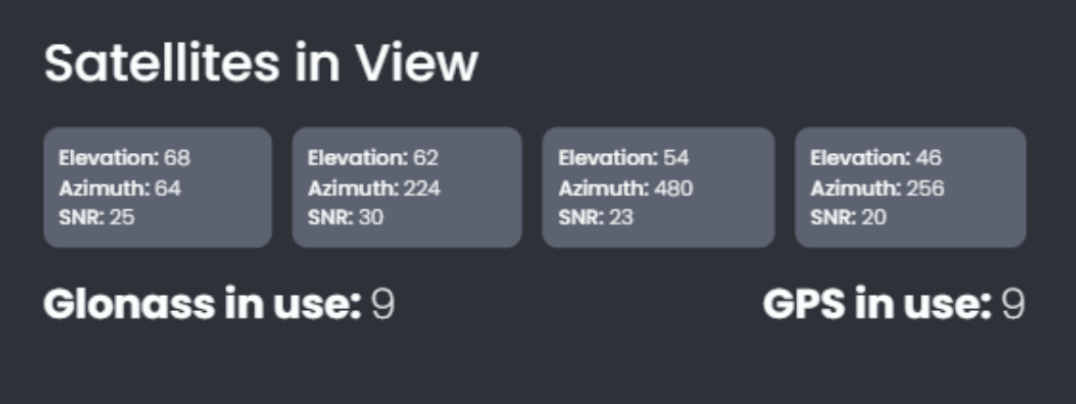
\includegraphics [scale=0.8] {ui_satellites_in_view}
    \centering
    \captionof{figure} {Satellites in View container in the dashboard}
\end{figure}

\subsubsection{Graphs}
The user interface displays two types of graphs: trend graphs and gauge graphs.

The type of graph used to display information depends on the nature of the data being represented. Trend graphs 
plot data where it may be useful to see historical points to determine a trend in the measurements, and gauge graphs are 
used for values which don't necessarily need to be viewed in past context.

To display the data on gauges and trend graphs, the ApacheECharts library for React was used. The trend graph components use
mission time as their $x$ series, and a specific data packet as their $y$ series (such as altitude).

Graph components are made re-usable by parameterizing the key data that will change. A list of parameters given to a trend
graph component is the following:
\footnote{Note: This is not an exhaustive list of parameters, but rather a selection of them.}:

\begin{multicols}{2}
    \begin{itemize} 
        \item Graph title    
        \item Units of measurement (for both axes)       
        \item Colour theme of the graph
        \item Axes titles
        \item List of $x$ values
        \item List of $y$ values
    \end{itemize}
\end{multicols}

\textbf{Trend Graphs}

Trend graphs are best suited for showing changes in data over time. The dashboard uses trend graphs
to represent velocity, acceleration and altitude. These values should be viewed in context of their historical values.
Each trend graphs has $n$ historical points represented at any moment, where $n$ is the number of historical points stored
in the local storage buffer. It is usually set to 20.

\begin{figure}[H]
    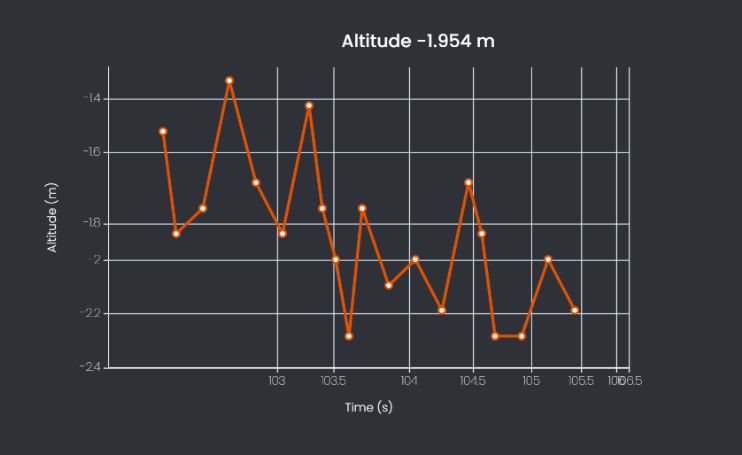
\includegraphics [scale=1] {ui_trend_graph}
    \centering
    \captionof{figure} {A trend graph displaying altitude over time of the rocket}
\end{figure}



\textbf{Gauge Graphs}

Gauge graphs are used to display a single value or data point at a specific moment in time and are best suited for
displaying real-time data that does not need historical context. The dashboard uses gauges for temperature and pressure.

To specify a range for each gauge chart, maximum and minimum value parameters are passed to the Gauge graph component.
The value displayed in the gauge meter is the most recently received packet of the value being displayed (i.e. temperature). 


\begin{figure}[H]
    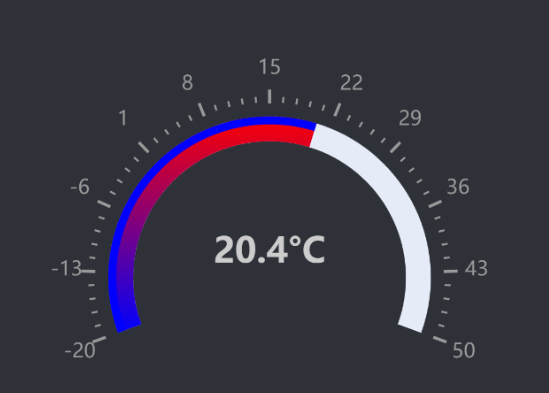
\includegraphics [scale=0.75] {ui_gauge_graph}
    \centering
    \captionof{figure} {A gauge graph displaying the temperature of the rocket}
\end{figure}

